% =====================================================================
%  J. Giorno -- Paper III (draft)
%  Belief-Driven Crash Risk: Wealth Effects, Filtered Regime Beliefs and
%  Feller--Tsallis Fear. Theory and Preliminary Evidence.
%  ONE self-contained file: the figure is drawn with pgfplots inside this
%  file and all references are written out at the end.
%  Compile: pdflatex Giorno_Paper_III_Draft.tex  (run twice)
% =====================================================================
\documentclass[11pt,a4paper]{article}

\usepackage[margin=2.5cm]{geometry}
\usepackage[T1]{fontenc}
\usepackage[utf8]{inputenc}
\usepackage{lmodern}
\usepackage{amsmath,amssymb,amsthm,mathtools}
\usepackage{enumitem}
\usepackage{booktabs}
\usepackage{tabularx}
\usepackage{threeparttable}
\usepackage{xcolor}
\usepackage{pgfplots}
\pgfplotsset{compat=1.17}
\usepackage[authoryear,round]{natbib}
\usepackage[colorlinks=true,linkcolor=blue!50!black,citecolor=blue!50!black,urlcolor=blue!50!black]{hyperref}

\newtheorem{theorem}{Theorem}
\newtheorem{proposition}{Proposition}
\newtheorem{corollary}{Corollary}
\newtheorem{lemma}{Lemma}
\newtheorem{prediction}{Prediction}
\theoremstyle{remark}
\newtheorem*{remark}{Remark}

\title{\textbf{Belief-Driven Crash Risk}\\[4pt]
\large Wealth Effects, Filtered Regime Beliefs and Feller--Tsallis Fear:\\
Theory and Preliminary Evidence}
\author{J.~Giorno, PhD\\[2pt]
\small Graduate Program in Economics, Maring\'a State University (UEM), Brazil\\
\small PhDRisk Ltda, Maring\'a, Brazil\\
\small \texttt{jgiorno@uem.br}}
\date{Draft --- 12 November 2026}

\begin{document}
\maketitle

\begin{abstract}
\noindent We develop a theory in which stock market crashes are partly endogenous and
their likelihood depends on the market's own perception of stress. Levered investors have
linear risk tolerance, written as a HARA utility in Tsallis $q$-exponential form, and share
a filtered belief that the economy is in a stressed regime. With constant absolute risk
aversion ($q=1$) the equilibrium price is unique and continuous, so every crash is
exogenous. With wealth effects, excess demand is a concave quadratic in price: a fold exists
exactly when $q$ exceeds a closed-form threshold $q^*$, which falls with leverage, and
crashes occur when a fundamental shock crosses the fold point. Whether greater fear moves
the fold closer depends on a wealth pivot at $W=1/\gamma$. The fear state follows a Feller
square-root jump-diffusion whose stationary law is Gamma, so the long-run probability that
the market is capable of a fold is a closed-form Gamma tail. A key implication is that,
when perceived stress is high, smaller or unclear news suffices to trigger a crash. Using
newspaper codings of 501 S\&P~500 crash days from 1928 to 2022, we find that the share of
crashes without a clear news cause rises from 26\% when predicted stress is low to 61\% when
it is high, robust to crash size and era; the effect weakens to marginal significance once
crisis continuation is controlled for. Tests of the leverage channel using FINRA margin
debt, and of convexity in the belief, are not supported. We report all designs tried and
state the theory's predictions so that they can be tested more deeply with better leverage
data.
\end{abstract}

\noindent\textbf{Keywords:} market crashes; wealth effects; HARA utility; Tsallis
statistics; Feller diffusion; regime switching; filtering; news and jumps.\\
\textbf{JEL:} G01, G12, G14, C58, D81.

% =====================================================================
\section{Introduction}

Large market falls often arrive without news that seems large enough to explain them.
\citet{BBDS2021} read next-day newspaper accounts of over 8,000 large daily moves in 19
national markets and found that a substantial share have no clear cause. This paper proposes
a theory of why, and when, that should happen.

The mechanism combines three familiar ingredients in a new way. First, investors who hold
the risky asset on leverage have \emph{wealth effects}: their risk tolerance rises and falls
with their wealth. Second, all investors observe the economy imperfectly and share a
\emph{filtered belief} $\pi_t$ that the economy is in a stressed regime. Third, fear itself
moves: after a crash, risk aversion rises and decays slowly. The single theoretical result
that ties these together is that wealth effects create a \emph{fold} in the equilibrium
price, and perceived stress moves the market towards that fold, so that a smaller shock is
enough to cause a discontinuous fall.

The paper makes four contributions.
\begin{enumerate}[leftmargin=*]
\item A closed-form characterisation of when the equilibrium price can fold
(Proposition~\ref{prop:fold}), showing that constant absolute risk aversion rules it out
(Proposition~\ref{prop:cara}) and that leverage lowers the threshold (Corollary~\ref{cor:lev}).
\item A sign result for fear: greater fear moves the fold closer only when levered wealth is
below a pivot (Proposition~\ref{prop:sign}), which follows from a wealth-pivot property of
the Tsallis $q$-exponential utility (Proposition~\ref{prop:pivot}).
\item A Feller (1951) square-root model of the fear state whose Gamma stationary law gives a
closed-form probability that the market is capable of a fold
(Proposition~\ref{prop:gamma}).
\item An identification result showing that a regime-switching jump model can only produce
an affine dependence of crash probability on beliefs (Lemma~\ref{lem:affine}), and
preliminary evidence from a century of crash news.
\end{enumerate}

We are explicit about what the evidence does and does not show. The belief channel receives
support in the long sample; the leverage channel and the convexity prediction do not, with
the data available to us. We regard this paper as stating a theory with sharp, falsifiable
predictions, and we set these out in Section~\ref{sec:future} for deeper testing.

% =====================================================================
\section{Related literature}

\begin{center}
\small
\begin{tabularx}{\textwidth}{>{\raggedright\arraybackslash}p{4.3cm}>{\raggedright\arraybackslash}X>{\raggedright\arraybackslash}X}
\toprule
Literature & What it does & What this paper adds \\
\midrule
HARA utility \citep{Merton1971,Pollak1971} & Linear risk tolerance; DARA with a wealth floor & Tsallis $q$-parameterisation; $q$ indexes wealth effects \\
Tsallis robust preferences \citep{MeyerGohde2019,Tian2022} & Tsallis entropy as a model-uncertainty foundation & Motivation for $q$; not claimed as new \\
Wealth and liquidity spirals \citep{GennotteLeland1990,KyleXiong2001,BrunnermeierPedersen2009} & Wealth or funding spirals amplify shocks & Closed-form fold; belief-indexed crash intensity \\
Learning about jump intensity \citep{Benzoni2011} & Agents learn an exogenous jump intensity & Jumps are endogenous folds; beliefs move the threshold \\
Square-root diffusions \citep{Feller1951,CIR1985} & Boundary classification; Gamma stationary law & Feller fear state; probability of fold capacity \\
Time-varying risk aversion \citep{CampbellCochrane1999,Cohn2015,GuisoSapienzaZingales2018} & Risk aversion rises after crises & Crash-excited fear with a wealth pivot \\
Jump news \citep{CutlerPoterbaSummers1989,BBDS2021} & Many large moves lack clear news & Predicts when unclear-news crashes are more frequent \\
Mutually exciting jumps \citep{Hawkes1971,AitSahalia2015} & Jumps propagate across markets & Propagated jumps as external shocks \\
\bottomrule
\end{tabularx}
\end{center}

% =====================================================================
\section{The model}

\subsection{The economy}

A risky asset in fixed supply $S$ has expected payoff $m(\pi)=m_0-\delta\pi$ ($\delta>0$)
and payoff variance $v$, where $\pi$ is the commonly filtered probability of the stressed
regime.
\begin{itemize}[leftmargin=*]
\item \textbf{Levered investors} hold $x_0$ shares and cash $c$ (negative $c$ means
leverage), so marked-to-market wealth is $W(P)=c+x_0P$. Their utility and risk tolerance
are
\begin{equation}
u_q(W)=-\big[1-(1-q)\gamma W\big]^{\frac{1}{1-q}},\qquad
T_q(W)=-\frac{u_q'}{u_q''}=\frac{1}{q\gamma}+\frac{q-1}{q}W,
\end{equation}
which is a HARA utility in Tsallis $q$-exponential form \citep{Tsallis1988,Tsallis2009};
$q\to1$ gives CARA. Their demand is $x(P)=T_q(W(P))\,(m(\pi)-P)/v$.
\item \textbf{Arbitrageurs} have limited capacity and linear demand $A(m_A-P)$, $A>0$.
\end{itemize}
Market clearing requires
\begin{equation}
Z(P;\pi)=T_q\big(W(P)\big)\frac{m(\pi)-P}{v}+A(m_A-P)-S=0 .
\end{equation}

\subsection{No wealth effects, no endogenous crashes}

\begin{proposition}[Uniqueness under CARA]\label{prop:cara}
If $q=1$, $Z$ is strictly decreasing in $P$, the equilibrium price is unique, and it is
continuous in $\pi$ and in fundamental shocks.
\end{proposition}
\begin{proof}
$T_1=1/\gamma$ is constant, so $\partial Z/\partial P=-1/(\gamma v)-A<0$; the unique root is
continuous in $m(\pi)$ by the implicit function theorem.
\end{proof}

\subsection{The fold in closed form}

Let $\alpha\equiv\frac{1}{q\gamma}+\frac{q-1}{q}c$ and $\beta\equiv\frac{q-1}{q}x_0$, so
$T_q=\alpha+\beta P$. Then $vZ=0$ is the quadratic
\begin{equation}
-\beta P^2+(\beta m-\alpha-Av)P+\alpha m+v(Am_A-S)=0,
\end{equation}
which has at most two roots and is concave in $P$ for $q>1$; the higher root is the stable
equilibrium.

\begin{proposition}[Fold existence and location]\label{prop:fold}
A fold exists if and only if
\[
q>q^*\equiv1+\frac{A/\gamma}{x_0(S-Am_A)-Ac}\qquad\big(\text{when } x_0(S-Am_A)-Ac>0\big).
\]
The fold point and fold price are
\[
m^*=\frac{Av-\alpha+2\sqrt{v\big(\beta(S-Am_A)-\alpha A\big)}}{\beta},\qquad
P^*=\frac{\beta m^*-\alpha-Av}{2\beta},
\]
and the fold is economically relevant when $P^*>0$ and $T_q(P^*)>0$.
\end{proposition}
\begin{proof}
The discriminant in $P$, $D(m)=(\beta m-\alpha-Av)^2+4\beta(\alpha m+v(Am_A-S))$, is
quadratic in $m$ with roots $m=[Av-\alpha\pm2\sqrt{v(\beta(S-Am_A)-\alpha A)}]/\beta$. These
are real iff $\beta(S-Am_A)>\alpha A$, i.e.\
$\frac1q[(q-1)(x_0(S-Am_A)-Ac)-A/\gamma]>0$. The high-price equilibrium exists above the
larger root, where the two equilibria merge at $P^*$.
\end{proof}

\begin{corollary}[Leverage lowers the fold threshold]\label{cor:lev}
$\partial q^*/\partial c>0$: more leverage (more negative $c$) lowers $q^*$.
\end{corollary}

\subsection{The wealth pivot and the sign of the fear effect}

\begin{proposition}[Wealth pivot]\label{prop:pivot}
For $A_q(W)=q\gamma/[1+(q-1)\gamma W]$,
$\partial A_q/\partial q=\gamma(1-\gamma W)/[1+(q-1)\gamma W]^2$. A rise in $q$ raises
absolute risk aversion if $W<1/\gamma$, lowers it if $W>1/\gamma$, and leaves $A_q=\gamma$
at $W=1/\gamma$ for every $q$.
\end{proposition}

\begin{proposition}[Sign of the fear effect]\label{prop:sign}
At a relevant fold, with $W^*=c+x_0P^*$,
\[
\frac{dm^*}{dq}=-\frac{(W^*-1/\gamma)(m^*-P^*)}{q^2\,T_q(W^*)},
\qquad\text{so}\qquad
\operatorname{sign}\frac{dm^*}{dq}=\operatorname{sign}\Big(\frac1\gamma-W^*\Big).
\]
\end{proposition}
\begin{proof}
At the fold $Z=0$ and $Z_P=0$, so $Z_m\,dm^*+Z_q\,dq=0$. Here $Z_m=T_q/v>0$ and, since
$\partial T_q/\partial q=(W-1/\gamma)/q^2$, $Z_q=(W^*-1/\gamma)(m^*-P^*)/(q^2v)$. Levered
investors are long at the fold, so $m^*-P^*>0$.
\end{proof}

\noindent We call $W^*<1/\gamma$ the \emph{fragile} state (more fear moves the fold closer)
and $W^*>1/\gamma$ the \emph{robust} state. An implication of Proposition~\ref{prop:pivot}
is that after a crash, investors below the pivot reduce exposure while those above it
increase it.

\subsection{Crash intensity}

Fundamental shocks $\varepsilon$ with density $f$ and survival function $\bar F$ arrive at
rate $\lambda_s$.

\begin{theorem}[Belief-driven crash intensity]\label{thm:curv}
\begin{enumerate}[label=(\roman*),leftmargin=*]
\item If $q=1$, there are no endogenous crashes.
\item If $q>q^*$, endogenous crashes arrive with intensity
$\lambda(\pi)=\lambda_s\,\bar F\big(m_0-\delta\pi-m^*(q)\big)$.
\item $\lambda''(\pi)=-\lambda_s\delta^2f'\big(m_0-\delta\pi-m^*(q)\big)$, so $\lambda$ is
convex in $\pi$ wherever the shock density is decreasing at the threshold; for Student-$t$
($q'$-Gaussian, $q'=(\nu+3)/(\nu+1)$; \citealp{deSouzaTsallis1997}) shocks this holds on
the whole relevant tail.
\item A rise in $q$ raises crash intensity in the fragile state and lowers it in the robust
state.
\end{enumerate}
\end{theorem}

\noindent Parts (i)--(iv) are proved for linear arbitrageur demand; extending them to concave
demand and adding a buyer of last resort to pin the post-crash price is left open. A direct
implication of (ii) is that \emph{the shock needed to trigger a crash shrinks as perceived
stress rises}; this is the prediction we test with news data in Section~\ref{sec:evidence}.

\noindent\textbf{Numerical verification.} For $\gamma=2$, $v=1$, $c=-0.3$, $x_0=1$,
$A=0.15$, $m_A=0.6$, $S=1$: with $q=1$ the price falls smoothly (largest step 0.004); with
$q=1.5$ it collapses by 0.91 at the fold. The closed form gives $q^*=1.079$ and $m^*=2.858$
at $q=1.5$ (grid search: 2.855). Across 17{,}093 randomly drawn relevant folds the sign in
Proposition~\ref{prop:sign} held in every case; both states occur.

% =====================================================================
\section{Feller--Tsallis fear}

The excess fear state $q_t-1>0$ follows a Feller square-root jump-diffusion:
\begin{equation}\label{eq:feller}
dq_t=\kappa_q(q_0-q_t)\,dt+\sigma_q\sqrt{q_t-1}\,dB^q_t+J_q\,dN_t,
\end{equation}
with baseline $q_0>1$, mean reversion $\kappa_q>0$, sentiment volatility $\sigma_q>0$,
$dB^q_t$ correlated with price innovations at $\rho_{Yq}\le0$, and upward fear jumps
$J_q\ge0$ at crash times. In daily data $dN_t$ is the Bernoulli crash indicator.

\begin{proposition}[Feller domain preservation]\label{prop:feller}
If $2\kappa_q(q_0-1)\ge\sigma_q^2$ and $J_q\ge0$, the CARA boundary $q=1$ is inaccessible;
between jumps $q_t-1$ has the noncentral chi-square transition density of \citet{CIR1985}.
\end{proposition}

\begin{proposition}[Gamma law and probability of fold capacity]\label{prop:gamma}
Without fear jumps, the stationary law of $q_t-1$ is Gamma with shape
$a_q=2\kappa_q(q_0-1)/\sigma_q^2$ and rate $r_q=2\kappa_q/\sigma_q^2$, so the long-run
probability that the market is capable of a fold is
\[
\Pr(q>q^*)=\frac{\Gamma\big(a_q,\,r_q(q^*-1)\big)}{\Gamma(a_q)} .
\]
The Feller condition is equivalent to $a_q\ge1$. With $J_q\ge0$ this is a lower bound (by a
comparison argument, to be verified). By Corollary~\ref{cor:lev}, higher leverage lowers
$q^*$ and raises this probability.
\end{proposition}

\begin{remark}
The Gamma boundary law parallels the result in \citet{Giorno1993}, obtained with It\^o
calculus in the tradition of \citet{LiptserShiryaev2001}. Numerically, with $\kappa_q=2$,
$q_0-1=0.5$, $\sigma_q=0.8$ and $q^*=1.6$, a simulated path gives $\Pr(q>q^*)=0.308$
against the Gamma tail $0.302$.
\end{remark}

\noindent In the fragile state a crash therefore raises future crash intensity through two
channels: the belief $\pi_t$ jumps upwards \citep{Wonham1964,Bremaud1981}, and fear $q_t$
jumps by $J_q$. They decay at different rates, set by regime persistence and by $\kappa_q$.

% =====================================================================
\section{Econometric identification}

In daily data, with returns $Y_t$ and predicted belief
$b^-_t=\pi_1+\kappa_M(b_{t-1}-\pi_1)$ from a two-state hidden Markov model
\citep{Hamilton1989},
\begin{equation}
Y_t=\mu_{K_t}+s_{K_t}X_t-B_tG_t,\qquad B_t\sim\mathrm{Bernoulli}\big(\varepsilon_{K_t}+\lambda(b^-_t)\big).
\end{equation}

\begin{lemma}[Affine equivalence]\label{lem:affine}
Under regime-dependent jumps only ($\lambda\equiv0$),
$\Pr(B_t=1\mid\mathcal F_{t-1})=\varepsilon_0+(\varepsilon_1-\varepsilon_0)b^-_t$. If the
regime diffusion densities coincide, an affine term $\lambda_1b$ gives the same one-step
predictive density with $\varepsilon_1+\lambda_1$ in place of $\varepsilon_1$, so it is only
weakly identified.
\end{lemma}
\begin{proof}[Proof sketch]
With $f_k(y;\varepsilon)=(1-\varepsilon)g_k(y)+\varepsilon J(y)$, the predictive density is
$p_0(y)+\lambda_1b[J(y)-(1-b)g_0(y)-bg_1(y)]$; if $g_0=g_1=g$ it equals
$(1-\bar\varepsilon)g+\bar\varepsilon J$ with
$\bar\varepsilon=\varepsilon_0+(\varepsilon_1+\lambda_1-\varepsilon_0)b$.
\end{proof}

\noindent Belief-driven crash risk is therefore identified through curvature in $b^-_t$, or
through auxiliary information that separates endogenous from exogenous crashes. News
clarity is such information: in the theory, an exogenous crash is triggered by a large,
clear shock regardless of fragility, while an endogenous crash needs only a small or unclear
shock once the market is close to the fold.

% =====================================================================
\section{Preliminary evidence}\label{sec:evidence}

\subsection{Data and construction}

Daily index levels for the S\&P~500 (1928--2026), the Ibovespa (1995--2026) and Bitcoin
(2014--2026) are from Yahoo Finance. Monthly margin debt is from FINRA's margin statistics
(1997--2026). Newspaper codings of US daily moves larger than 2.5\% in absolute value,
1900--2022, with cause and a continuous clarity index, are from \citet{BBDS2021}. The
predicted stress belief $b^-_t$ comes from a two-state Gaussian hidden Markov model fitted
by maximum likelihood; it is a simplification of the Student-$t$ jump model above, used here
for transparency. Leverage $L_t$ is margin debt relative to the index level (detrended and
standardised) or its 12-month excess growth, lagged two months to respect FINRA's
publication delay. Standard errors are from block bootstraps (63-day blocks) or, for
jump-day samples, case bootstraps. All results are reproduced by scripts listed in the
Appendix.

\subsection{Main result: the belief channel in crash news, 1928--2022}

Among 501 S\&P~500 downward jump days matched to the newspaper codings, we call a crash
\emph{low-clarity} if its clarity index is below the sample median. Conditional on a crash
occurring, the probability that it is low-clarity rises with the predicted stress belief
(probit coefficient 0.99, $z=5.6$). Figure~\ref{fig:clarity} shows the pattern.

\begin{figure}[ht]
\centering
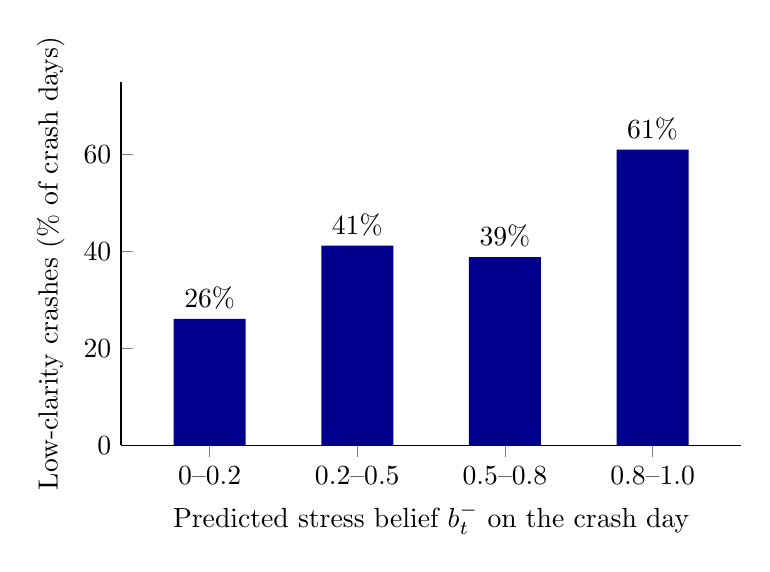
\begin{tikzpicture}
\begin{axis}[
  ybar, bar width=26pt, width=0.78\textwidth, height=6.2cm,
  ymin=0, ymax=75, ylabel={Low-clarity crashes (\% of crash days)},
  xlabel={Predicted stress belief $b^-_t$ on the crash day},
  symbolic x coords={0--0.2,0.2--0.5,0.5--0.8,0.8--1.0}, xtick=data,
  nodes near coords={\pgfmathprintnumber[fixed,precision=0]{\pgfplotspointmeta}\%},
  axis lines*=left, enlarge x limits=0.2, fill=blue!55!black, draw=none,
  ymajorgrids=false]
\addplot[fill=blue!55!black,draw=none] coordinates {(0--0.2,26.1) (0.2--0.5,41.2) (0.5--0.8,38.8) (0.8--1.0,61.0)};
\end{axis}
\end{tikzpicture}
\caption{Share of S\&P~500 downward jumps (moves below $-2.5\%$) that newspapers attribute to
no clear cause, by the predicted stress belief on the day, 1928--2022. Number of crash days
per bin: 88, 51, 67, 295. Clarity codings from \citet{BBDS2021}.}
\label{fig:clarity}
\end{figure}

\begin{table}[ht]
\centering
\begin{threeparttable}
\caption{Probability that a crash is low-clarity, given a crash: robustness}
\label{tab:robust}
\small
\begin{tabular}{lcc}
\toprule
Specification & Coefficient on $b^-_t$ & $z$ \\
\midrule
$b^-_t$ only & 0.987 & 5.56 \\
+ crash size relative to recent volatility & 0.947 & 4.56 \\
+ era dummies (1946--96, 1997--2022) & 0.820 & 3.70 \\
+ linear time trend & 0.814 & 3.68 \\
+ crisis continuation (jump in previous 5 days) & 0.441 & 1.68 \\
First crashes only (no jump in previous 5 days), $n=276$ & 0.493 & 1.62 \\
\bottomrule
\end{tabular}
\begin{tablenotes}\footnotesize
\item Probit on crash days. Size is $|r_t|/\hat\sigma_{t-1}$ with an EWMA ($\lambda=0.94$)
volatility. The continuation dummy has coefficient 0.446 ($z=3.11$). Among first crashes the
low-clarity share is 30.3\% when $b^-_t\le0.5$ ($n=132$) and 45.8\% when $b^-_t>0.5$
($n=144$).
\end{tablenotes}
\end{threeparttable}
\end{table}

The pattern holds within each era: the low-clarity share rises from 47\% to 75\% (1928--45),
from 30\% to 49\% (1946--96) and from 20\% to 27\% (1997--2022) between low ($b^-_t\le0.5$)
and high ($b^-_t>0.5$) stress. It also holds within each third of the crash-size
distribution. However, Table~\ref{tab:robust} shows that controlling for crisis
continuation halves the coefficient and reduces it to marginal significance. Part of the
effect is therefore crashes that follow other crashes without new news. That is itself what
the theory's self-excitation predicts, but it is also what one would observe if journalists
simply had nothing new to report in the middle of a sell-off; our data cannot separate the
two.

In the daily panel, the probability of a low-clarity crash rises with $b^-_t$ (linear term
1.77, $z=4.43$) without significant curvature (LR test of the quadratic term 0.30), while
clear-news crashes rise and then flatten (quadratic term $-1.50$, $z=-4.20$). The theory's
convexity prediction (Theorem~\ref{thm:curv}(iii)) is therefore not confirmed.

\subsection{The leverage channel: not supported with FINRA margin debt}

We tested whether the belief curvature of crash probability rises with leverage (the
coefficient on $(b^-_t)^2L_t$) on the S\&P~500, 1997--2026, in a grid fixed in advance: three
jump thresholds and two leverage measures. Table~\ref{tab:lev} reports every cell.

\begin{table}[ht]
\centering
\begin{threeparttable}
\caption{Leverage--curvature interaction, S\&P~500 1997--2026}
\label{tab:lev}
\small
\begin{tabular}{llccc}
\toprule
Leverage measure & Jump threshold & Jump days & $(b^-)^2\times L$ ($z$) & LR \\
\midrule
Detrended level & $-2.5\sigma$ & 126 & $-0.09$ ($-0.86$) & 0.82 \\
Detrended level & $-3\sigma$ & 71 & $-0.13$ ($-1.11$) & 1.13 \\
Detrended level & $-4\sigma$ & 22 & $\phantom{-}0.03$ ($0.08$) & 0.02 \\
Excess growth & $-2.5\sigma$ & 120 & $-0.16$ ($-1.37$) & 2.66 \\
Excess growth & $-3\sigma$ & 69 & $-0.11$ ($-0.80$) & 0.87 \\
Excess growth & $-4\sigma$ & 21 & $\phantom{-}0.18$ ($0.61$) & 1.01 \\
\bottomrule
\end{tabular}
\begin{tablenotes}\footnotesize
\item Daily probit of jump days on $b^-_t$, $(b^-_t)^2$, $L_t$ and $(b^-_t)^2L_t$; jumps
are returns below $-k$ times the previous day's EWMA volatility. LR is the likelihood-ratio
statistic for the interaction (5\% critical value 3.84).
\end{tablenotes}
\end{threeparttable}
\end{table}

None of the interactions is significant and four of six have the wrong sign. Splitting
1997--2022 crashes by news clarity does not change this: the interaction is $-0.24$
($z=-1.33$) or $0.07$ ($z=0.33$) for low-clarity crashes, depending on the leverage measure.
We see two explanations. FINRA margin debt measures retail brokerage leverage at monthly
frequency, whereas the investors near a fold in a crash are mostly levered institutions;
or the leverage channel is weak in US equities. The first can be tested with intermediary
leverage \citep{AdrianEtulaMuir2014} or with crypto-derivatives open interest.

\subsection{Other evidence}

\begin{itemize}[leftmargin=*]
\item \textbf{Curvature without leverage.} On Bitcoin (2014--2026) and the S\&P~500
(1991--2026), the quadratic belief term is positive in all six threshold choices but never
significant (largest LR 2.71), and crash frequency is U-shaped in the belief rather than
rising. A volatility-relative jump definition likely inflates the low-belief end.
\item \textbf{Bitcoin liquidations.} Of the ten largest Bitcoin liquidation days since 2021,
including \$19.2 billion on 10 October 2025, only two occurred at high predicted stress
($b^-_t>0.7$); several followed strong rallies. This is consistent with the leverage channel
(a fold approached through leverage built in calm markets), which a returns-based belief
cannot see.
\item \textbf{Propagation.} The Ibovespa's crash rate is 0.60\% on all days but 21.9\% on
S\&P~500 crash days, and 37\% of Ibovespa crashes coincide with a US crash, close to the
38\% attribution to US news found by \citet{BBDS2021}. Propagated crashes are external shocks
for the receiving market, which suggests a ``same shock, different fragility'' design.
\end{itemize}

% =====================================================================
\section{Predictions for deeper testing}\label{sec:future}

The theory makes the following predictions. We state them so that researchers with better
data can test them directly.

\begin{prediction}[Belief channel]\label{pred:belief}
Conditional on a crash, the probability that it lacks a clear news cause increases with the
market's perceived stress. \emph{Status:} supported 1928--2022; marginal after controlling
for crisis continuation.
\end{prediction}

\begin{prediction}[Leverage channel]
The sensitivity of crash probability to perceived stress is larger when levered investors are
closer to their wealth floor. \emph{Status:} not supported with FINRA margin debt; untested
with institutional leverage.
\end{prediction}

\begin{prediction}[Convexity]
Endogenous crash intensity is convex in perceived stress (Theorem~\ref{thm:curv}(iii)).
\emph{Status:} not confirmed; requires a likelihood model with an explicit jump component.
\end{prediction}

\begin{prediction}[Fear sign]
After a crash, further crashes cluster beyond what the belief channel explains only when
levered wealth is below the pivot (Proposition~\ref{prop:sign}); and investors below the
pivot sell while those above it buy (Proposition~\ref{prop:pivot}). \emph{Status:} untested.
\end{prediction}

\begin{prediction}[Same shock, different fragility]
When an external shock (a crash abroad) hits several markets, the markets that crash are those
with higher perceived stress and leverage. \emph{Status:} untested.
\end{prediction}

\noindent The most informative data would be: (i) daily intermediary or hedge-fund leverage;
(ii) daily open interest and liquidations in crypto derivatives, where leverage is observed
directly; (iii) investor-category flows around crashes, for example from B3 in Brazil; and
(iv) news codings for markets other than the US. A likelihood model with regime-specific
Student-$t$ diffusion and a Bernoulli--Gamma jump component would test convexity properly.

% =====================================================================
\section{Conclusion}

Wealth effects make equilibrium prices capable of folding, and perceived stress brings the
market closer to the fold. The theory delivers closed forms for when a fold exists, how
leverage and fear move it, and the long-run probability that a market is fragile. A century
of crash news supports one of its central implications: crashes without clear news are more
common when perceived stress is high, although part of this reflects crisis continuation.
The leverage and convexity predictions remain open. We offer them as a precise agenda for
deeper testing.

% =====================================================================
\appendix
\section{Reproducibility}

All numbers in Section~\ref{sec:evidence} are produced by the following scripts, run on the
data described above:
\begin{itemize}[leftmargin=*]
\item \texttt{paper3\_fold\_closed\_form.py}: closed-form fold, random check of
Proposition~\ref{prop:sign};
\item \texttt{paper3\_feller\_gamma\_check.py}: Gamma tail of the fear state;
\item \texttt{e1\_quick.py}: leverage--curvature grid (Table~\ref{tab:lev});
\item \texttt{e1\_curvature.py}: curvature tests on Bitcoin and the S\&P~500;
\item \texttt{e1\_news.py}: news-clarity split, 1997--2022;
\item \texttt{e1\_news\_long.py}: news-clarity results, 1928--2022
(Figure~\ref{fig:clarity}, Table~\ref{tab:robust}).
\end{itemize}
Two data caveats: B3 spreadsheets exported to Excel swap day and month when the day is 12
or less; and FINRA free-credit balances are reported as a single combined figure before
February 2010.

% =====================================================================
\begin{thebibliography}{99}
\small

\bibitem[Adrian et~al.(2014)]{AdrianEtulaMuir2014}
Adrian, T., Etula, E., and Muir, T. (2014). Financial intermediaries and the cross-section
of asset returns. \emph{Journal of Finance}, 69(6), 2557--2596.

\bibitem[A\"it-Sahalia et~al.(2015)]{AitSahalia2015}
A\"it-Sahalia, Y., Cacho-Diaz, J., and Laeven, R.~J.~A. (2015). Modeling financial
contagion using mutually exciting jump processes. \emph{Journal of Financial Economics},
117(3), 585--606.

\bibitem[Baker et~al.(2021)]{BBDS2021}
Baker, S.~R., Bloom, N., Davis, S.~J., and Sammon, M.~C. (2021). What triggers stock market
jumps? NBER Working Paper No.~28687 (revised April 2025).

\bibitem[Benzoni et~al.(2011)]{Benzoni2011}
Benzoni, L., Collin-Dufresne, P., and Goldstein, R.~S. (2011). Explaining asset pricing
puzzles associated with the 1987 market crash. \emph{Journal of Financial Economics},
101(3), 552--573.

\bibitem[Br\'emaud(1981)]{Bremaud1981}
Br\'emaud, P. (1981). \emph{Point Processes and Queues: Martingale Dynamics}. New York:
Springer.

\bibitem[Brunnermeier and Pedersen(2009)]{BrunnermeierPedersen2009}
Brunnermeier, M.~K., and Pedersen, L.~H. (2009). Market liquidity and funding liquidity.
\emph{Review of Financial Studies}, 22(6), 2201--2238.

\bibitem[Campbell and Cochrane(1999)]{CampbellCochrane1999}
Campbell, J.~Y., and Cochrane, J.~H. (1999). By force of habit: A consumption-based
explanation of aggregate stock market behavior. \emph{Journal of Political Economy}, 107(2),
205--251.

\bibitem[Cohn et~al.(2015)]{Cohn2015}
Cohn, A., Engelmann, J., Fehr, E., and Mar\'echal, M.~A. (2015). Evidence for
countercyclical risk aversion: An experiment with financial professionals. \emph{American
Economic Review}, 105(2), 860--885.

\bibitem[Cox et~al.(1985)]{CIR1985}
Cox, J.~C., Ingersoll, J.~E., and Ross, S.~A. (1985). A theory of the term structure of
interest rates. \emph{Econometrica}, 53(2), 385--407.

\bibitem[Cutler et~al.(1989)]{CutlerPoterbaSummers1989}
Cutler, D.~M., Poterba, J.~M., and Summers, L.~H. (1989). What moves stock prices?
\emph{Journal of Portfolio Management}, 15(3), 4--12.

\bibitem[de Souza and Tsallis(1997)]{deSouzaTsallis1997}
de Souza, A.~M.~C., and Tsallis, C. (1997). Student's $t$- and $r$-distributions: Unified
derivation from an entropic variational principle. \emph{Physica A}, 236(1--2), 52--57.

\bibitem[Feller(1951)]{Feller1951}
Feller, W. (1951). Two singular diffusion problems. \emph{Annals of Mathematics}, 54(1),
173--182.

\bibitem[Gennotte and Leland(1990)]{GennotteLeland1990}
Gennotte, G., and Leland, H. (1990). Market liquidity, hedging, and crashes.
\emph{American Economic Review}, 80(5), 999--1021.

\bibitem[Giorno(1993)]{Giorno1993}
Giorno, J. (1993). \emph{Quantum of Knowledge}. PhD dissertation. [Institution to be
completed.]

\bibitem[Guiso et~al.(2018)]{GuisoSapienzaZingales2018}
Guiso, L., Sapienza, P., and Zingales, L. (2018). Time varying risk aversion. \emph{Journal
of Financial Economics}, 128(3), 403--421.

\bibitem[Hamilton(1989)]{Hamilton1989}
Hamilton, J.~D. (1989). A new approach to the economic analysis of nonstationary time
series and the business cycle. \emph{Econometrica}, 57(2), 357--384.

\bibitem[Hawkes(1971)]{Hawkes1971}
Hawkes, A.~G. (1971). Spectra of some self-exciting and mutually exciting point processes.
\emph{Biometrika}, 58(1), 83--90.

\bibitem[Kyle and Xiong(2001)]{KyleXiong2001}
Kyle, A.~S., and Xiong, W. (2001). Contagion as a wealth effect. \emph{Journal of Finance},
56(4), 1401--1440.

\bibitem[Liptser and Shiryaev(2001)]{LiptserShiryaev2001}
Liptser, R.~S., and Shiryaev, A.~N. (2001). \emph{Statistics of Random Processes}, Vols.~I
and II, 2nd ed. Berlin: Springer.

\bibitem[Merton(1971)]{Merton1971}
Merton, R.~C. (1971). Optimum consumption and portfolio rules in a continuous-time model.
\emph{Journal of Economic Theory}, 3(4), 373--413.

\bibitem[Meyer-Gohde(2019)]{MeyerGohde2019}
Meyer-Gohde, A. (2019). Generalized entropy and model uncertainty. \emph{Journal of Economic
Theory}, 183, 312--343.

\bibitem[Pollak(1971)]{Pollak1971}
Pollak, R.~A. (1971). Additive utility functions and linear Engel curves. \emph{Review of
Economic Studies}, 38(4), 401--414.

\bibitem[Tian(2022)]{Tian2022}
Tian, D. (2022). Pricing principle via Tsallis relative entropy in incomplete market.
arXiv:2201.05316; to appear in \emph{SIAM Journal on Financial Mathematics}.

\bibitem[Tsallis(1988)]{Tsallis1988}
Tsallis, C. (1988). Possible generalization of Boltzmann--Gibbs statistics. \emph{Journal of
Statistical Physics}, 52(1--2), 479--487.

\bibitem[Tsallis(2009)]{Tsallis2009}
Tsallis, C. (2009). \emph{Introduction to Nonextensive Statistical Mechanics: Approaching a
Complex World}. New York: Springer.

\bibitem[Wonham(1964)]{Wonham1964}
Wonham, W.~M. (1964). Some applications of stochastic differential equations to optimal
nonlinear filtering. \emph{SIAM Journal on Control}, 2(3), 347--369.

\end{thebibliography}

\end{document}
